\section{Improvements of the CEM-Optimizer}
\label{sec:cem_improv}
In the model-predictive control setting, the action sequences found by the optimizer can be very different between execution real-world times steps. For example at one time step the optimizer might find a pushing action leading towards the goal and in the next time step it determines a grasping action to be optimal to reach the goal. Na\"{i}ve replanning at every time step can then result in alternating between a pushing and a grasping attempt indefinitely causing the agent to get stuck and not making any progress towards to goal. 

%%SL.10.15: It's not clear whether this is done in every experiment or just some experiments.
We can resolve this problem by modifying the sampling distribution of the first iteration of CEM so that the optimizer commits to the plan found in the previous time step. In the simplest version of CEM the sampling distribution at first iteration of CEM is chosen to be a Gaussian with diagonal covariance matrix and zero mean. We instead use the best action sequence found in the optimization of the \emph{previous} real-world time step as the mean for sampling new actions in the \emph{current} real-world time-step. Since this action sequence is optimized for the previous time step we only use the values $a_{2:T}$ and omit the first action. To sample actions close to the action sequence from the previous time step we reduce the entries of the diagonal covariance matrix for the first $T-1$ time steps. It is crucial that the last entry of the covariance matrix at the end of the horizon is not reduced otherwise no exploration could happen for the last time step causing poor performance at later time steps.

\section{Experimental Setup}
\label{sec:experiment_setup}
To train both our video-prediction and registration models, we collected 20,000 trajectories of pushing motions and 15,000 trajectories with gripper control, where the robot randomly picks and moves objects using the grasping reflex described in section \ref{sec:system}. The data collection process is fully autonomous, requiring human intervention only to change out the objects in front of the robot. The action space consisted of relative movements of the end-effector in cartesian space along the $x$, $y$, and $z$ axes, and for some parts of the dataset we also added azimuthal rotations of the gripper and a grasping action.

\section{Experimental Evaluation}

\subsection{Experiments with multiple-objects rearrangement with occlusion}

 \autoref{fig:goingaroundocclusion} \todo{change this}shows an example of the SNA model successfully predicting the position of the obstacle through an occlusion and finding a trajectory that avoids the obstacle. 

\begin{figure*}
	\centering
	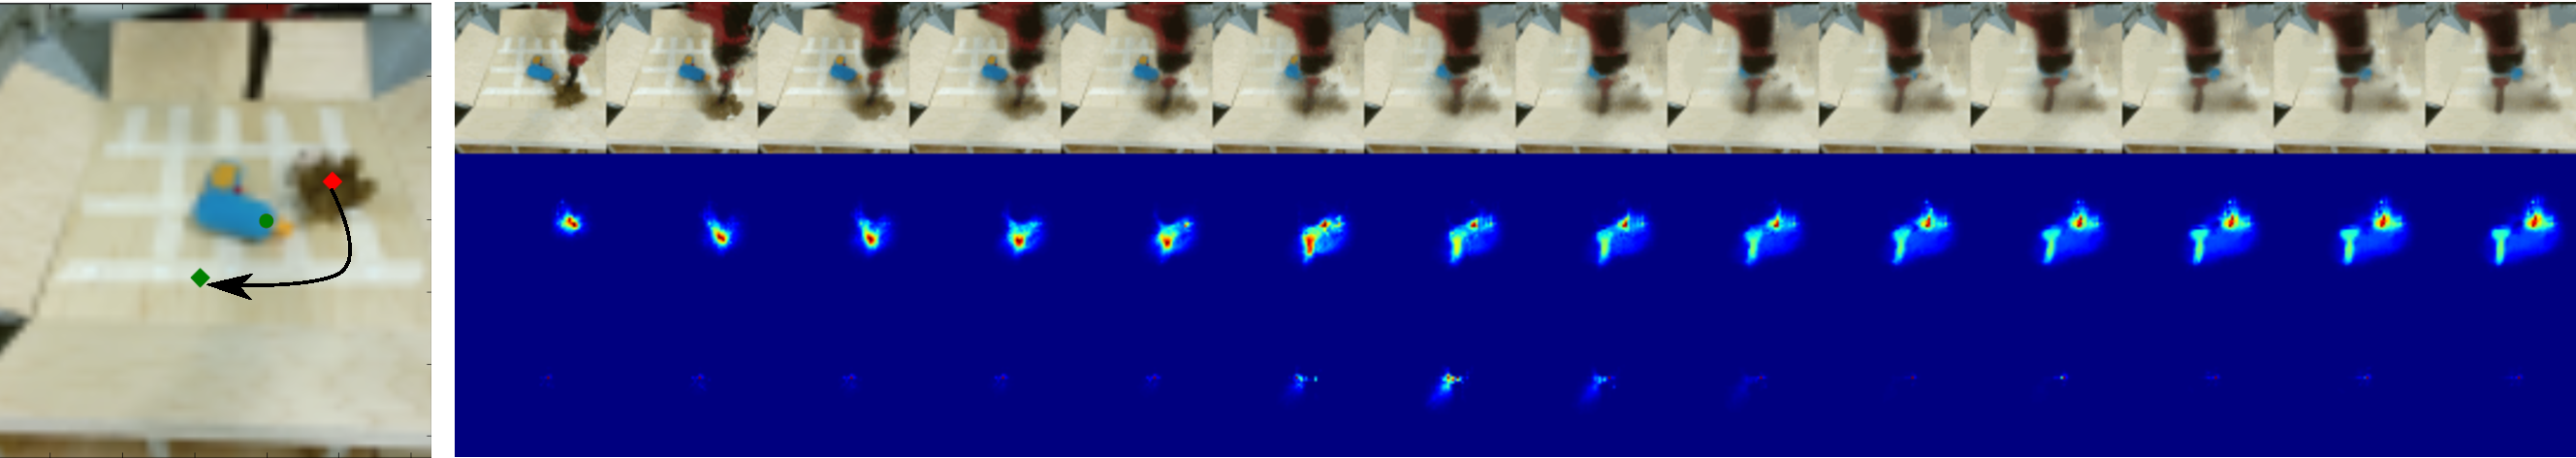
\includegraphics[width=1\linewidth]{images_sna/multiobject_qualitative/avoid_obstacle.pdf}
	\caption{Left: Task setup with green dot marking the obstacle. Right, first row: the predicted frames generated by SNA. Second row: the probability distribution of the designated pixel on the \textit{moving} object (brown stuffed animal). Note that part of the distribution shifts down and left, which is the indicated goal. Third row: the probability distribution of the designated pixel on the obstacle-object (blue power drill). Although the distribution increases in entropy during the occlusion (in the middle), it then recovers and remains on its original position.
		\label{fig:goingaroundocclusion}}
\end{figure*}


\subsection{Experiments with classifier-based cost function}
\begin{figure*}
	\centering
	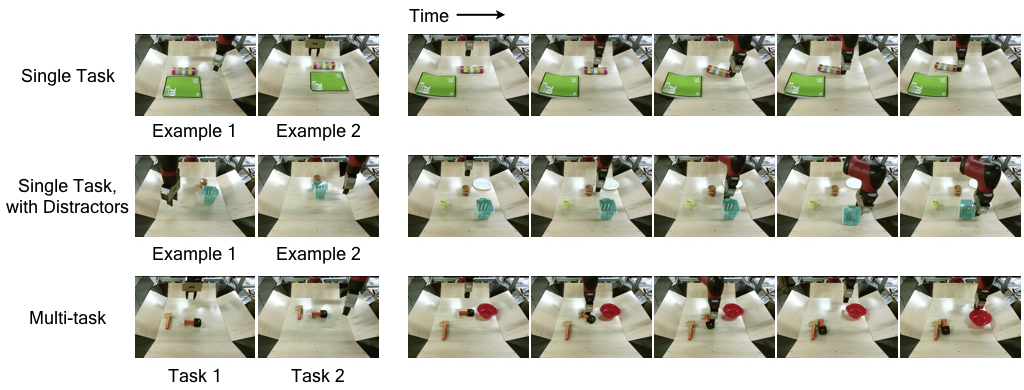
\includegraphics[width=0.8\textwidth]{images_cls/cls_results.jpeg}
	\caption{\small Object arrangement performance of our goal classifier with distractor objects and with two tasks. The left shows a subset of the 5 positive examples that are provided for inferring the goal classifier(s), while the right shows the robot executing the specified task(s) via visual planning. \todo{can go to appendix! classifier example wi}}
	\label{fig:cls_results}
	\vspace{-0.3cm}
\end{figure*}

\section{Simulated Experiments}
%\todo{shorten if necessary}

In order to provide a more controlled comparison, we also set up a realistic simulation environment using MuJoCo \cite{todorov2012mujoco}, which includes a robotic manipulator controlled via Cartesian position control, similar to our real world setup, pushing randomly-generated L-shaped objects with random colors (see details in supplementary materials). 
We trained the same video prediction model in this environment, and set up 50 evaluation tasks where blocks must be pushed to target locations with maximum episode lengths of 120 steps. 
We  compare our proposed registration-based method, ``predictor propagation,'' and ground-truth registration obtained from the simulator, which provides an oracle upper bound on registration performance. \autoref{fig:sim_bench} shows the results of this simulated evaluation, where the x-axis shows different distance thresholds, and the y-axis shows the fraction of evaluation scenarios where each method pushed the object within that threshold. We can see that, for thresholds around 0.1, our method drastically outperforms predictor propagation (i.e., prior work~\cite{sna}), and has a relatively modest gap in performance against ground-truth tracking. This indicates that our registration method is highly effective in guiding visual MPC, despite being entirely self-supervised.




